\documentclass[a4paper,12pt]{article}

\usepackage{graphicx}
\usepackage{ucs}
\usepackage[utf8x]{inputenc}
\PrerenderUnicode{åäöÅÄÖ}

\title{Costanza Userguide}
\author{M. Green, P. Krupinski, P. Melke, P. Sahlin, H. Jonsson}

\begin{document}

\maketitle

%\abstract 

\section{Introduction}

This document describes how to use COnfocal STack ANalyZer Application
(Costanza), an ImageJ\cite{Abramoff2004} plugin for analyzing confocal
stacks. The main purpose of Costanza is to segment nuclei marked cells
in three dimensions, making available quantitative measures such as
positions, sizes, and average intensities of GFP markers for the
segmented compartments. The main algorithm is independent of intensity
thresholds, allowing for segmentation of data of varying intensity.

Costanza assumes a greyscale stack of images as input, and work with
real length units and x, y, and z scales should be provided either via
ImageJ, or set by the user.

\section{Installation instructions}

In order to use Costanza you must have ImageJ
(http://rsb.info.nih.gov/ij) installed on your system. Unzip the
Costanza archive in the plugins directory of your ImageJ installation. Next
time you start ImageJ the plugin will show up as Costanza in the Plugins drop
down menu.

\section{Algorithms}

The algorithms privided in Costanza can be divided into the main
segmenter algorithm, preprocessing, and postprocessing.

\subsection{Steepest gradient descent for segmentation}



\subsection{Preprocessing}

\subsubsection{Intensity inversion}

Costanza assumes bright objects in a dark background. If the objects
are dark in a bright surrounding, the stack should be inverted. This
algorithm replaces each voxel intensity $I$ with its inverted value
$I_{max}-I$, where $I_{max}$ is the maximal value allowed in the
greyscale images. This algorithm does not require any user provided
parameter values.

\subsubsection{Background extraction by thresholding}

It may be benficial to remove voxels from treatment by the
segmentation algorithm. Both to remove uninteresting regions of the
stack, and for speeding up the algorithms. The background can be
extracted via a threshold filter, that assigns all voxels with
intensity $I$ less than a threshold value $I_{threshold}$ to belong to
the background, and will not be treated in the algorithms. The user
has to provide a value for the parameter $I_{threshold}$.

\subsubsection{Mean filter for smoothing}

Important for the segmentation to work is that the intensity noise is
low and the stack provided is smooth. This can be done by different
filters in ImageJ, but Costanza also provides a 3D filter for
smoothing. It uses a spherical XXX and replaces each voxel intensity
$I$ by an average calculated from all voxels with a center positioned
within a radius $R_{max}$ measured in real length. Since it can be
beneficial to run the filter multiple times with smaller $R_{max}$,
the user shopuld provide the two parameters, $R_{max}$ and the number
of times to run the filtering.

\subsection{Postprocessing}

\subsubsection{Peak removal}

\subsubsection{Peak merging}

\section{User interface}

\section{Examples}

The performance of the Costanza application is dependent on the
parameters given to the different algorithms used. Here we provide
some examples of applications where also the parameter values used are
presented to guide users into setting reasonable parameter values.

\subsection{SAM nuclei data in 3D}

This data set represents nuclei marked cells in the Arabidopsis shoot apical
meristem. The data set consists of a stack with 20 images, but here the result
will be displayed in 2D images for an easier check on performance. The
segmentation is run using two different resolutions, and the result is shown
in Fig.~\ref{fig:43zoom}.

\begin{figure}[h!]
\begin{center}

\includegraphics[width=0.25\columnwidth]{figures/43smallzoomCenters.eps}
\hspace{0.20\columnwidth}
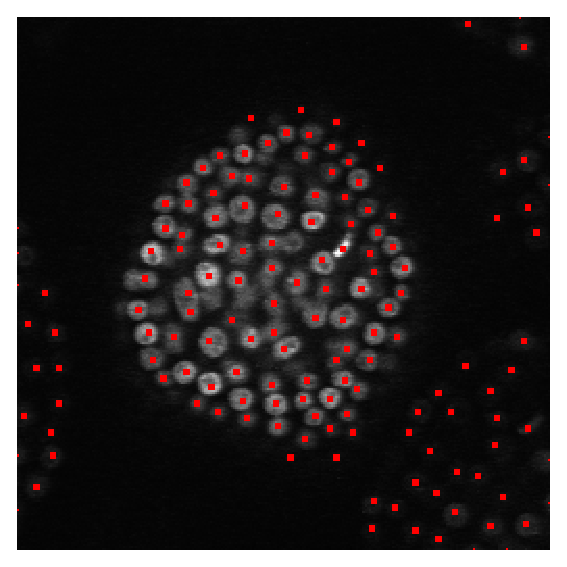
\includegraphics[width=0.5\columnwidth]{figures/43zoomCenters.eps}
\caption{Result shown for images of nuclei data. Original images can be found
	at http://www.thep.lu.se/...}
\label{fig:43zoom}
\end{center}
\end{figure}
%
Parameters used for these two runs are given in Table~\ref{tab:43zoom}, and
represents reasonable values also for 3D stacks.

\begin{table}
	\begin{center}
		\begin{tabular}{|l|cc|}
			\hline
			Parameter & Small & Large\\
			\hline
			Bg threshold & 10 & 10\\
			MeanFilter R & 1.0 & 2.5\\
			MeanFilter num & 2 & 2\\
			Remove Int Th. & 10 & 10\\
			Remove Size Th. & 5 & 10\\
			Merger R & 3 & 6\\
			xy-scale & 1 & 1\\
			z-scale & 1 & 2\\
			\hline
		\end{tabular}
		\caption{Nuclei extraction in 2D and 3D.}
		\label{tab:43zoom}
	\end{center}
\end{table}

\subsection{SAM membrane data in 2D}

This data set represents membrane marked cells in the Arabidopsis shoot apical
meristem. The data set consists of single images. The segmentation is run
using two different resolutions, and the result is shown in
Fig.~\ref{fig:membrane}.

\begin{figure}[h!]
\begin{center}
%\includegraphics[width=0.25\columnwidth]{figures/wus.eps}
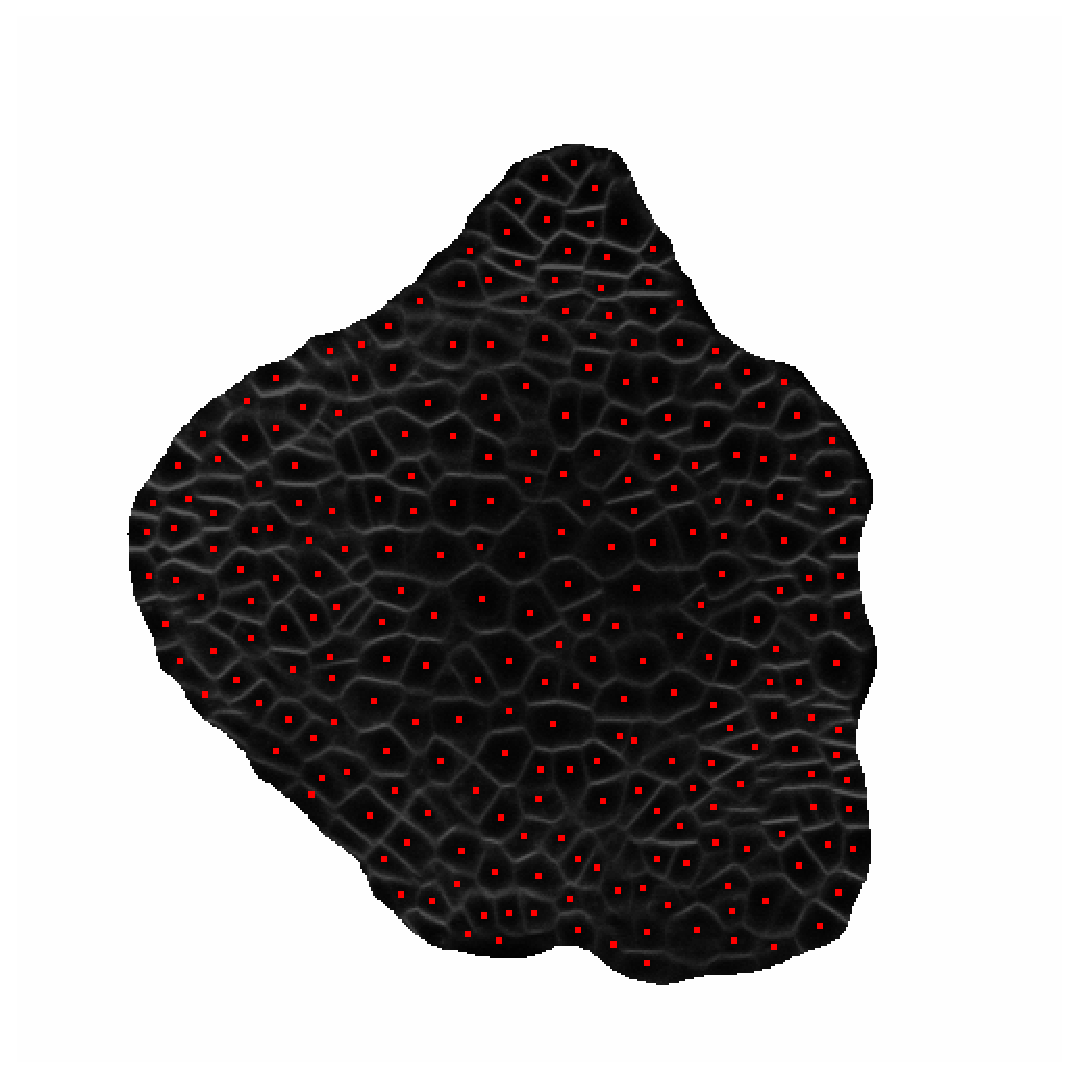
\includegraphics[width=0.25\columnwidth]{figures/wusCenters.eps}
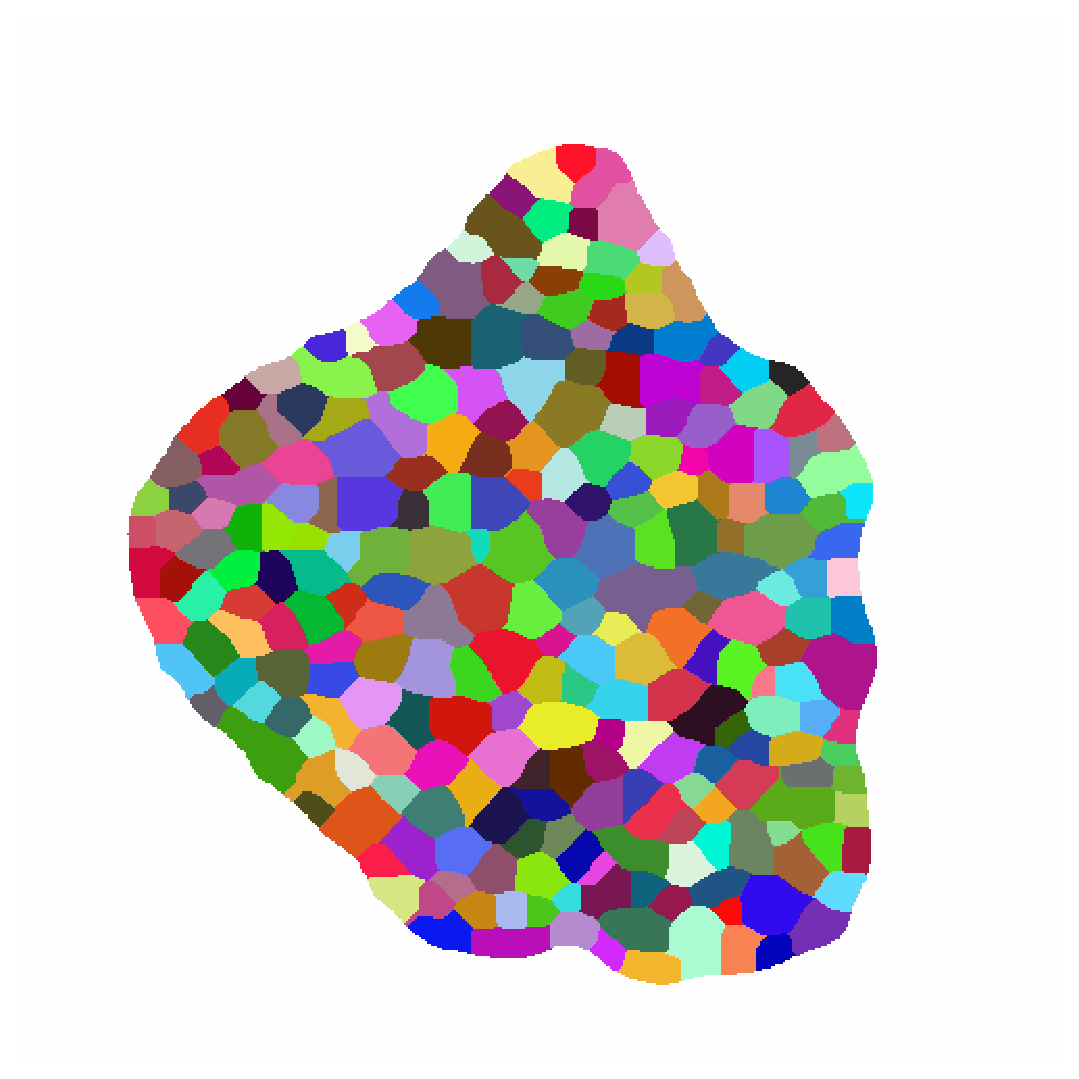
\includegraphics[width=0.25\columnwidth]{figures/wusBOAs.eps}
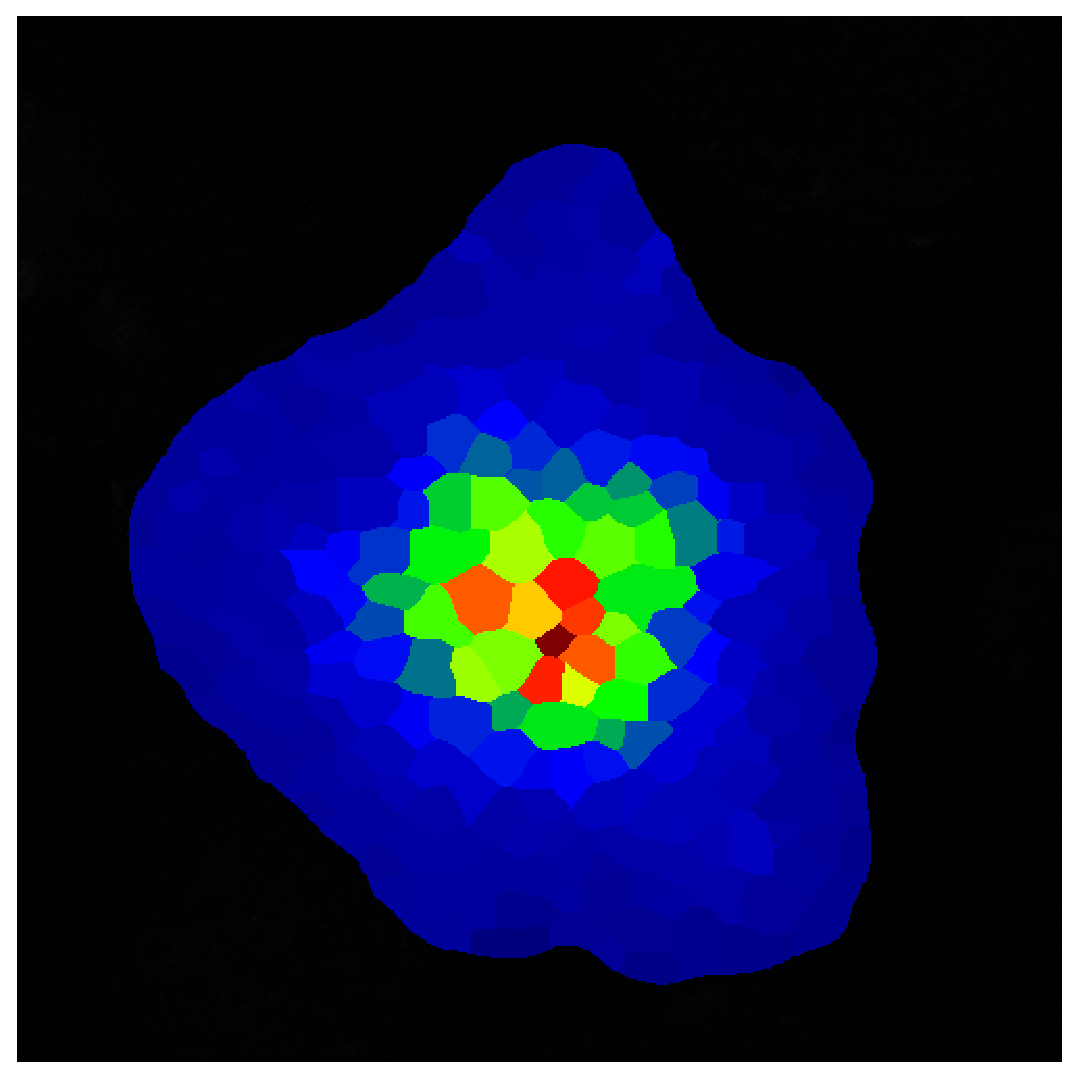
\includegraphics[width=0.25\columnwidth]{figures/wusBOAsIntensity.eps}

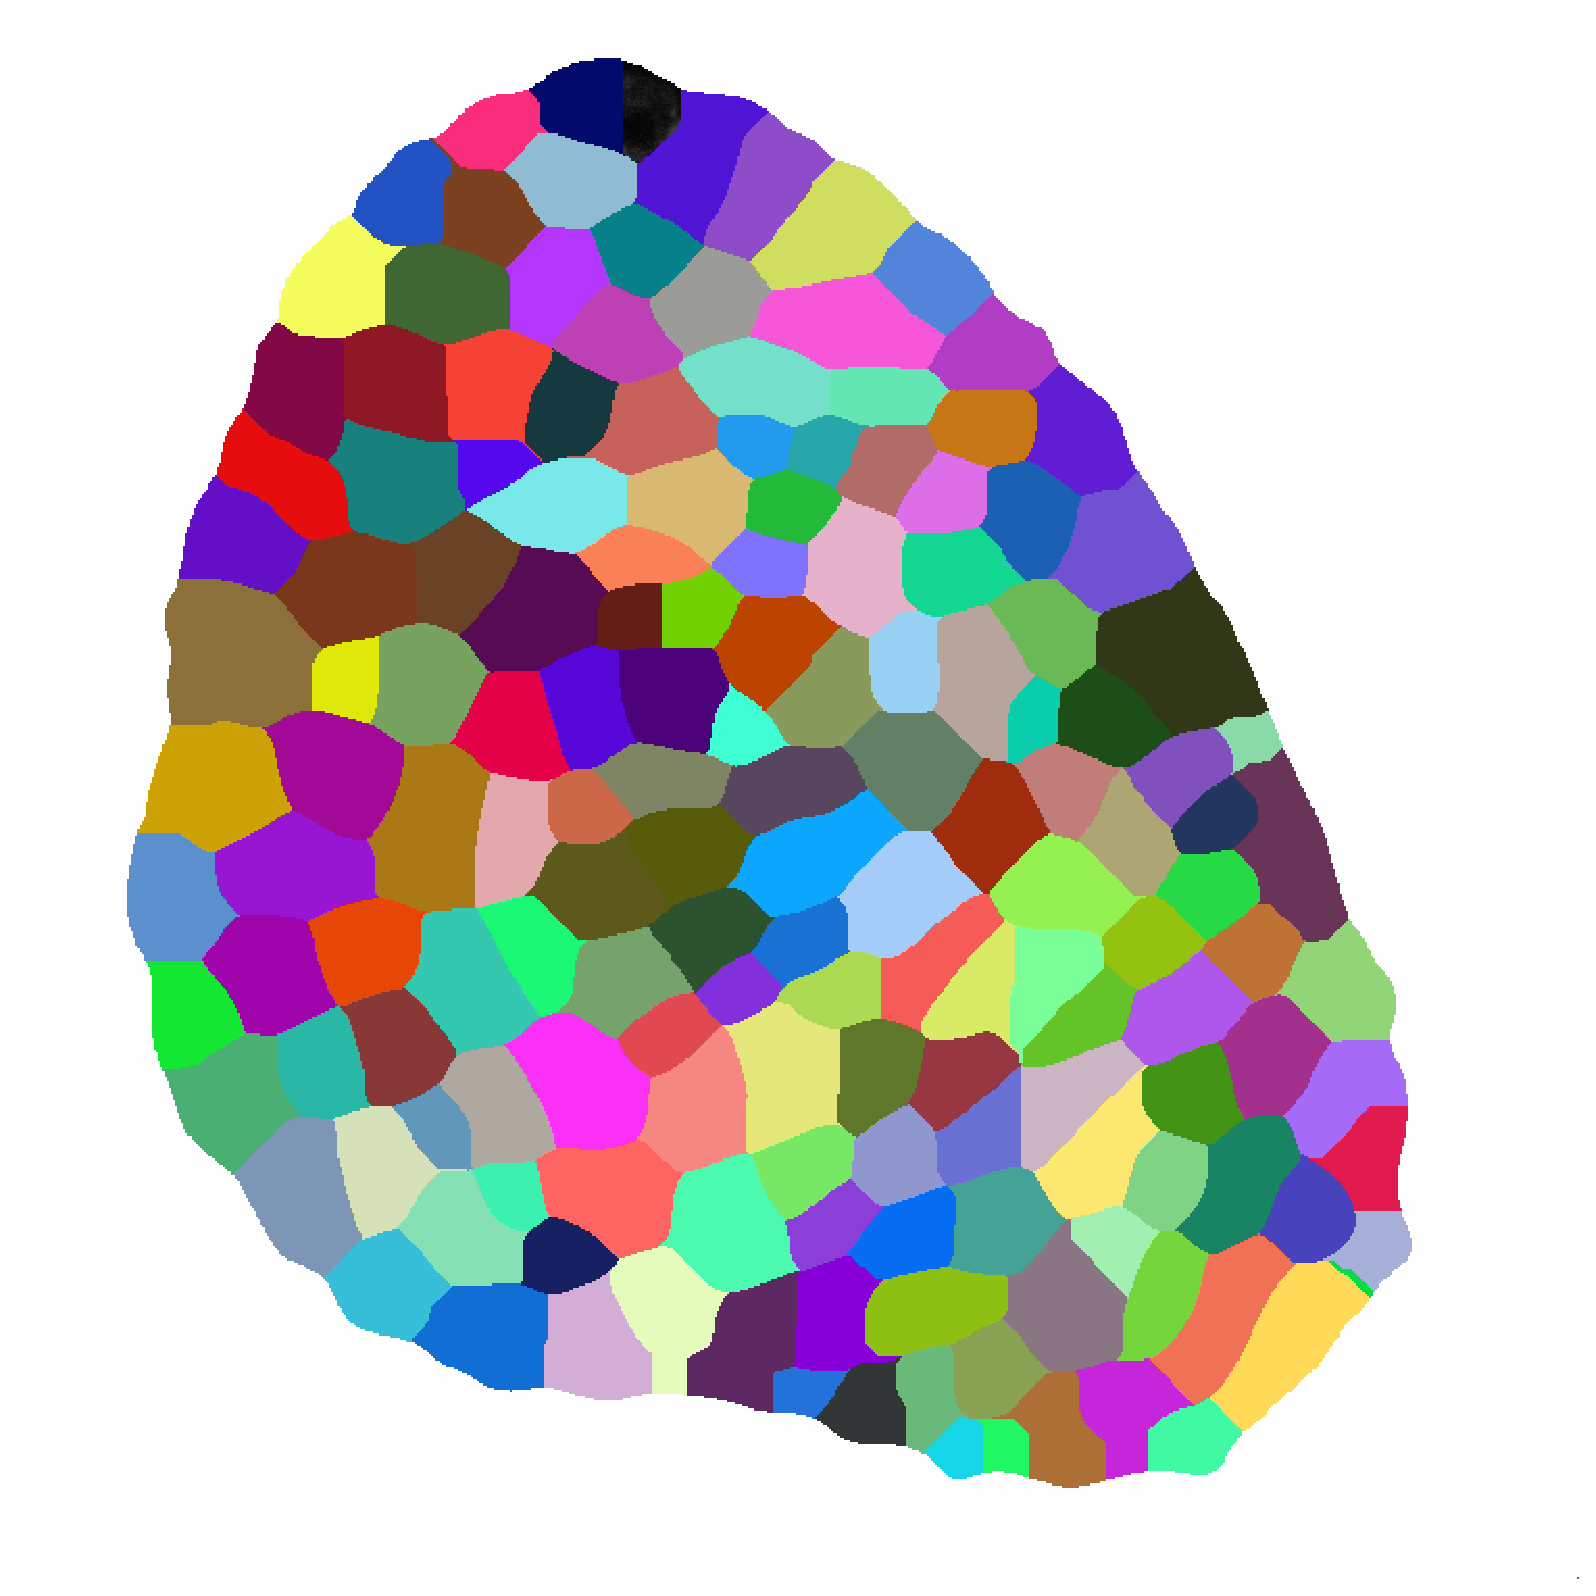
\includegraphics[width=0.33\columnwidth]{figures/pin1BOAs.eps}
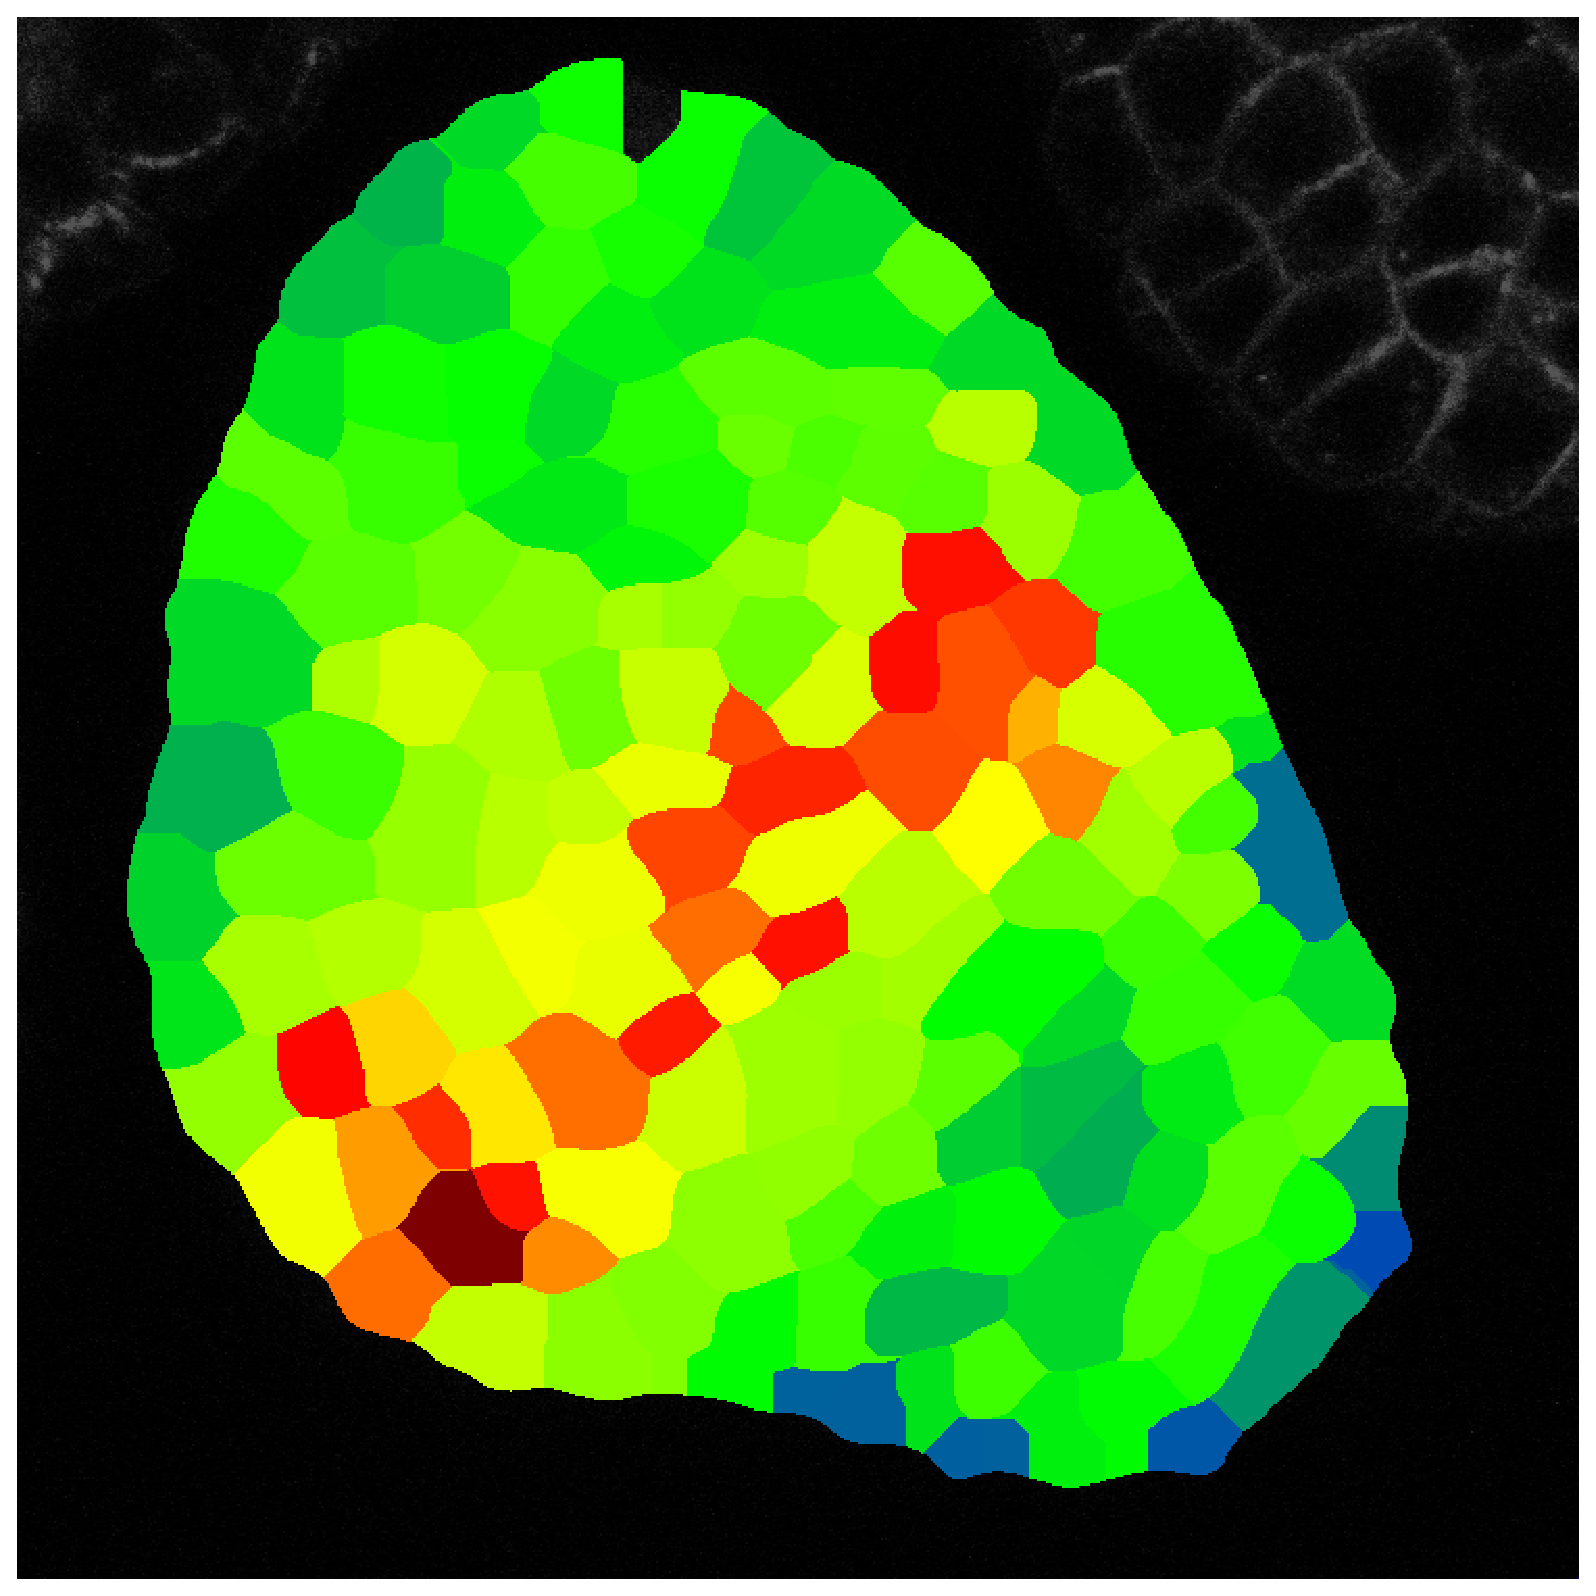
\includegraphics[width=0.33\columnwidth]{figures/pin1BOAsIntensity.eps}

\caption{Result shown for images of membrane data. Original images can be
	found at http://www.thep.lu.se/...}
\label{fig:membrane}
\end{center}
\end{figure}
%
Parameters used for these two segmentations are given in Table~\ref{tab:membrane}.

\begin{table}
	\begin{center}
		\begin{tabular}{|l|cc|}
			\hline
			Parameter & WUS & PIN1\\
			\hline
			Bg threshold & 1 & 1\\
			MeanFilter R & 5.0 & 10.0\\
			MeanFilter num & 2 & 2\\
			Remove Int Th. & 10 & 10\\
			Remove Size Th. & 10 & 10\\
			Merger R & 5 & 10\\
			xy-scale & 1 & 1\\
			z-scale & - & -\\
			\hline
		\end{tabular}
		\caption{Cell extraction in 2D membrane data.}
		\label{tab:membrane}
	\end{center}
\end{table}

\bibliographystyle{abbrv}
\bibliography{references}

\end{document}
